\section{Geometry --- not method family --- selects the compressor (E3)}
\label{sec:e3}

\begin{intuition}
\textbf{What this experiment tests.} If cluster geometry is the
organising variable, the choice between consolidation (cluster-aware
summaries) and learned vector quantization (cluster-agnostic codes)
should be predicted by $\deff_{\mathrm{local}}$, not by method-family
preference. E3 tests that. At matched bytes per vector, consolidation
Pareto-dominates PQ, OPQ, LSH, PCA+int8, and HNSW-prune on the five
corpora where $\deff_{\mathrm{local}} \lesssim 30$, and
learned quantization overtakes it on the one corpus where
$\deff_{\mathrm{local}} = 107.5$ (arXiv titles). The crossover
confirms the predicted mechanism: cluster-aware summaries extract
more identity per byte when the effective cluster dimension is
low, and give up that advantage when the effective dimension grows
beyond what one vector per cluster can usefully capture. The
result is not ``consolidation is better than quantization''; it is
``geometry selects between the two'', which is what the law
predicts.
\end{intuition}

\subsection{Experimental design}
\label{sec:e3:design}

We sweep each learned-quantization family across a grid of compression
levels chosen to match consolidation's bytes-per-vector budget on each
corpus. The grids:

\begin{itemize}[leftmargin=1.8em, itemsep=2pt]
\item \textbf{PQ}: $m \in \{4, 8, 16, 32\}$ code chunks, $256$
centroids per chunk (FAISS).
\item \textbf{OPQ}: same chunk schedule as PQ, plus a learned
rotation (FAISS).
\item \textbf{LSH}: signed random projections to
$\{64, 128, 256, 512\}$ bits, then reconstruct by the projection's
transpose.
\item \textbf{PCA + int8}: principal components to
$\{16, 32, 64, 128\}$ dimensions, then per-dimension int8 quantisation.
\item \textbf{HNSW-prune}: hnswlib index with $M = 16$, $ef = 200$,
and prune-and-rank at $\{25\%, 50\%, 75\%\}$ retention.
\end{itemize}

Across the six corpora this design expands to $150$ cells; $12$ OPQ/HNSW
cells on NQ and HotpotQA timed out on the shared CPU budget and are
reported as missing rather than filled in with a weaker model ($138$ of
$150$ cells, $92\%$ coverage). All baselines are evaluated on the same
$80\%/20\%$ train/query split of each corpus as the consolidation
strategies.

We measure \emph{bytes per vector} as the figure of merit on the
$x$-axis and identity accuracy on the $y$-axis, then overlay the five
consolidation strategies (each at its native compression level) as
stars on the same axes.

\subsection{Headline result}
\label{sec:e3:result}

Figure~\ref{fig:e3} shows the resulting Pareto frontiers per corpus. The
qualitative shape is consistent across five of the six corpora.

\paragraph{Low-to-moderate $\deff_{\mathrm{local}}$: consolidation wins.}
On DRM, the centroid star sits at identity $0.94$ at about $1$ KB per
vector, while PQ's frontier saturates near $0.80$ even at large
budget. On MS MARCO the centroid achieves $0.90$ against PQ's $0.85$
at matched compression. On HotpotQA the centroid is at $0.50$ and the
entire quantization family caps at $0.45$. The pattern: when
$\deff_{\mathrm{local}}$ is moderate (below $\approx 30$), the
cluster-aware summary extracts more identity per byte than
vector-wise quantization does. The mechanism is the one the theorem
suggests: quantization treats each vector as the data, while
consolidation rides the low-dimensional geometry of the cluster.

\paragraph{High-$\deff_{\mathrm{local}}$: quantization takes over.} On
arXiv titles ($\deff_{\mathrm{local}} = 107.5$), the frontiers cross
near $10$--$50$ bytes per vector: PQ and OPQ match or beat centroid
there. This is the predicted crossover: in the high-$\deff$ regime the
cap-volume bound is near-vacuous and no one-vector cluster summary can
compete with a well-trained quantizer. The crossover \emph{location}
is not something our theorem predicts quantitatively (the spread-regime
$c_1$ is vacuous, \S\ref{sec:e1:calibration}); the fact that the
crossover happens on the high-$\deff$ corpus and nowhere else is the
qualitative prediction we claim.

\paragraph{LSH, PCA+int8, HNSW-prune are dominated by PQ/OPQ.} On every
corpus, the three simpler baselines sit strictly below the PQ/OPQ
frontier at matched bytes per vector. This is consistent with the
general literature: PQ with a learned codebook dominates random
projections with the same bit
budget~\cite{johnson2019faiss,jegouPQ2011}. We include them because
they appear in production stacks, not because we expected them to beat
PQ.

\subsection{Reading E3 through the law}
\label{sec:e3:takeaway}

The scientific content of E3 is not a per-corpus recommendation but
the observation that \emph{a single geometric quantity,
$\deff_{\mathrm{local}}$, predicts which compression family wins}.
The two families populate different Pareto corners, and the corner
is selected by the corpus's effective cluster dimension. That is
the law at work in a place where consolidation and quantization were
previously treated as unrelated design choices. For practitioners, a
shorthand follows: on corpora where $\deff_{\mathrm{local}} \lesssim
30$ (most chat-style RAG content we have inspected), the fixed
centroid Pareto-dominates; on corpora where $\deff_{\mathrm{local}}
> 50$ (technical titles, code, diverse long-form), learned vector
quantization is the better choice. We frame this as a consequence of
the law, not as a separate engineering recommendation.

\begin{figure}[h]
\centering
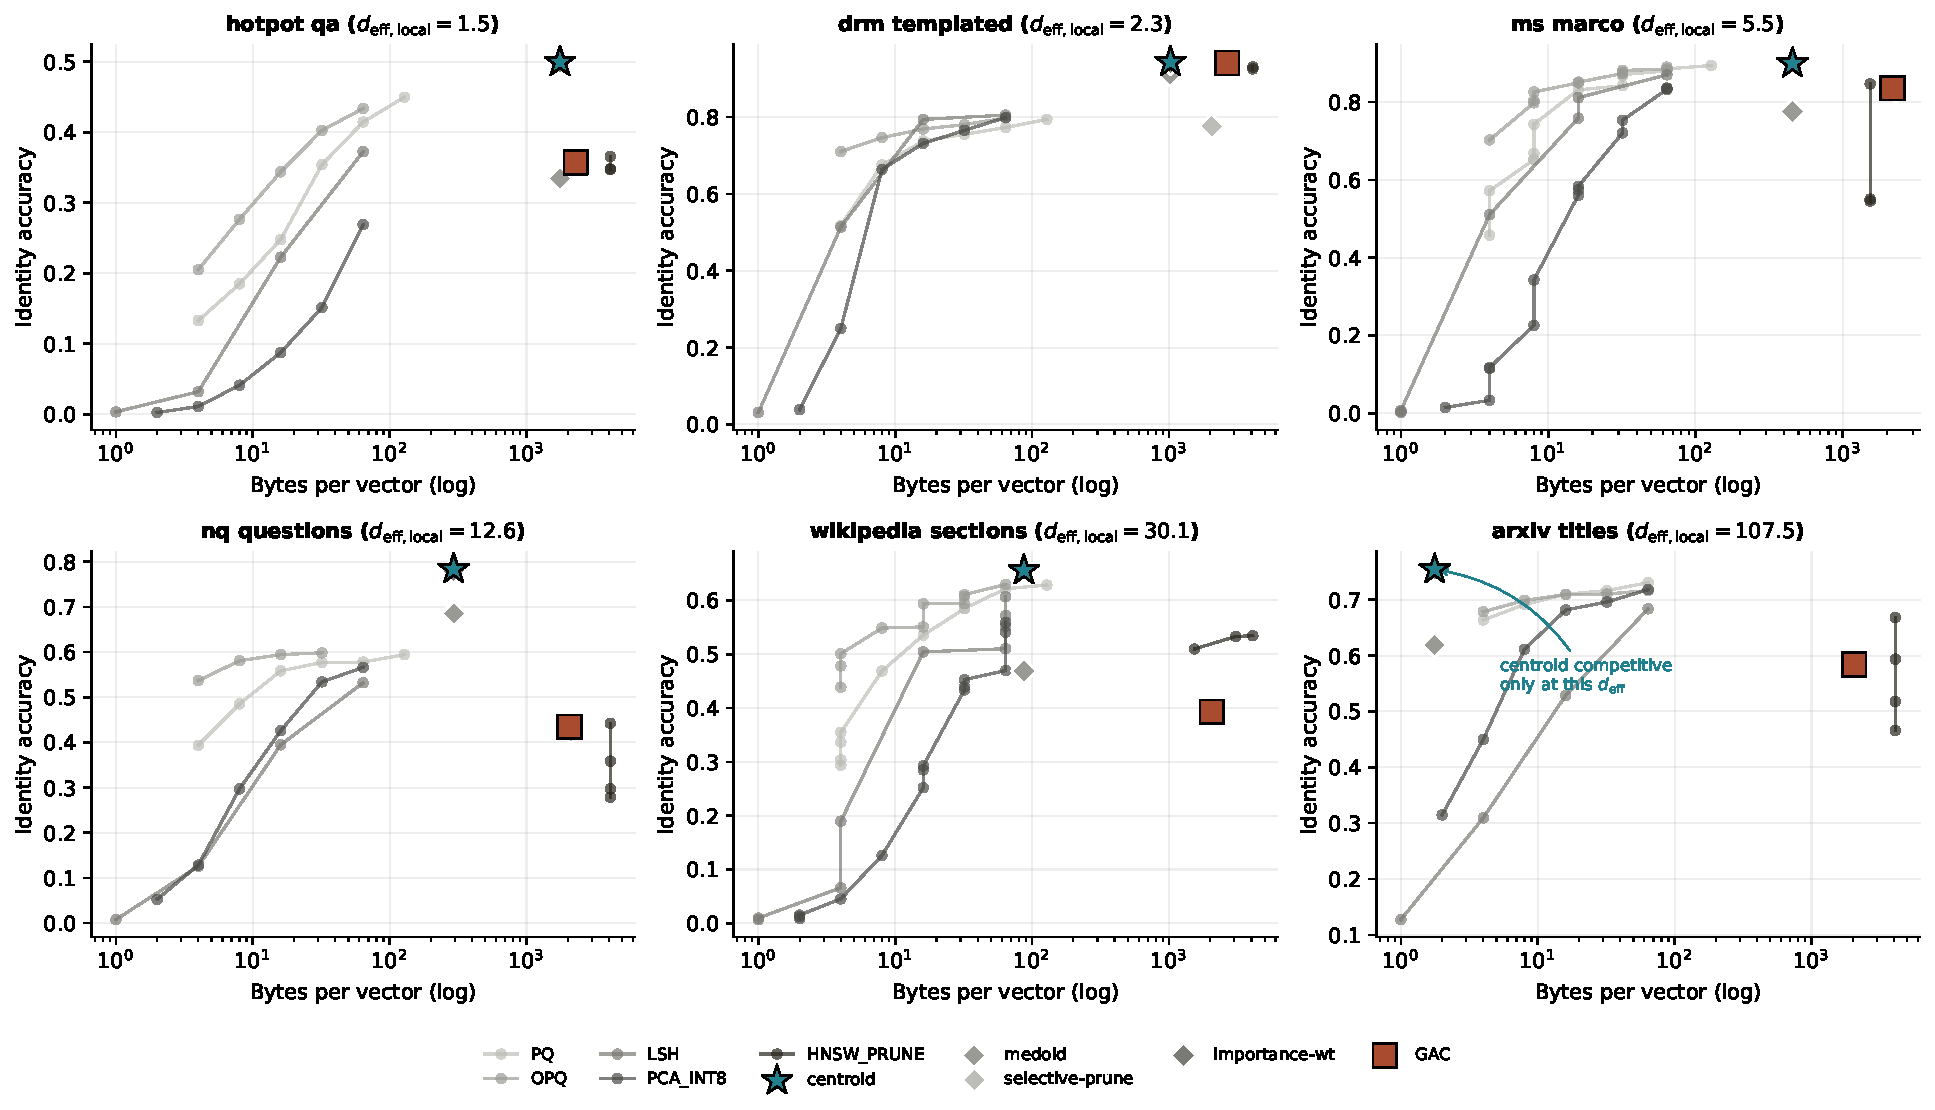
\includegraphics[width=0.98\linewidth]{figs/fig3_learned_baselines.pdf}
\caption{\textbf{Which compression family wins is a function of
$\deff_{\mathrm{local}}$, not of method choice.} Identity accuracy
versus bytes per vector (log scale) on six corpora, ordered by
$\deff_{\mathrm{local}}$. Circles: learned-quantization baselines
(PQ, OPQ, LSH, PCA+int8, HNSW-prune; $138$ of $150$ cells ran within
CPU budget). Stars: consolidation strategies at matched bytes. The
frontiers cross only on the corpus where $\deff_{\mathrm{local}} >
100$ (arXiv titles); on the other five, consolidation Pareto-dominates.
The crossing is annotated explicitly.}
\label{fig:e3}
\end{figure}
